%% Adaptado de 
%% http://www.ctan.org/tex-archive/macros/latex/contrib/IEEEtran/
%% Traduzido para o congresso de IC da USP
%%*****************************************************************************
% não modificar

\documentclass[twoside,conference,a4paper]{IEEEtran}

%******************************************************************************
% não modificar
\usepackage{IEEEtsup} % Definições complementares e modifica��es.
\usepackage[latin1]{inputenc} % Disponibiliza acentos.
\usepackage[english,brazil]{babel}
%% Disponibiliza Inglês e Português do Brasil.
\usepackage{latexsym,amsfonts,amssymb} % Disponibiliza fontes adicionais.
\usepackage{theorem} 
\usepackage[cmex10]{amsmath} % Pacote matemático básico 
\usepackage{url} 
%\usepackage[portuges,brazil,english]{babel}
\usepackage{graphicx}
\usepackage{amsmath}
\usepackage{amssymb}
\usepackage{color}
\usepackage[pagebackref=true,breaklinks=true,letterpaper=true,colorlinks,bookmarks=false]{hyperref}
\usepackage[tight,footnotesize]{subfigure} 
\usepackage[noadjust]{cite} % Disponibiliza melhorias em citações.
\usepackage{listings}
\usepackage{todonotes}
%%*****************************************************************************

\begin{document}
\selectlanguage{brazil}
\renewcommand{\IEEEkeywordsname}{Palavras-chave}

%%*****************************************************************************

\urlstyle{tt}
% Indicar o nome do autor e o curso/nível (grad-mestrado-doutorado-especial)
\title{MO810 - Trabalho 2}
\author{%
 \IEEEauthorblockN{Mateus Coradini Santos\,\IEEEauthorrefmark{1}}
 \IEEEauthorblockA{\IEEEauthorrefmark{1}%
				   Prof (a): Profa. Dra. Esther Luna Colombini \\
                   Aluno especial - Mestrado \\
                   E-mail: mateuscoradini@gmail.com}				   
}

%%*****************************************************************************

\maketitle

%%*****************************************************************************
% Resumo do trabalho
\begin{abstract}
O objetivo inicial deste trabalho são os testes das teorias aplicadas em sala de aula, colocando em pratica a implementação do sistema de controle diferencial para um robo movel executado em um ambiente simulado, no caso, usamos o software V-REP. Foram implementados dois comportamentos de controle \textit{Avoid Obstacle} e \textit{Wall Follow} utilizando sistemas Fuzzy em Java e estimativa de Pose baseada em odometria.
As classes de controle para os algoritmos em Fuzzy, foram implementadas a modo de fazer somentes testes básicos de implementação e não houve um trabalho de modelagem especifica para obter melhores resultados, pois o objetivo do trabalho era entender e aprender a utilizar a lógica em função das tarefas executadas anteriormente como malha aberta. A odometria não está correta, e ainda necessita de tratamento, pois não esta limpando os erros acumulados.
Os algoritmos de fuzzy para WallFollow e AvoidObstacle se encontram sem otimização no momento.

\end{abstract}

% Indique três palavras-chave que descrevem o trabalho
\begin{IEEEkeywords}
 V-REP Pioneer AvoidObstacleColision WallFollow Fuzzy
\end{IEEEkeywords}

%%*****************************************************************************
% Modifique as seções de acordo com o seu projeto

\section{Introdução}

Este projeto consiste no desenvolvimento de um sistema com inteligencia necessária para o controle do modelo de robo \textit{Pioneer P3-DX} no simulador \textit{V-REP}. A implementação foi realizada em Java versão 1.7, com a utilização de algumas bibliotecas como JFuzzyLite. Os ciclos de leitura e atuação dos sensores são controlados por threads na qual utilizamos um tempo de 300ms para atuação. O código fonte pode ser obtido em https://github.com/mateuscoradini/VRepSimulator/V2. As instruções de instalação se encontram na pagina principal, mapeados para MAC-OS e Windows. 

Este artigo está dividido em três sessões principais, cada uma com sua apresentação e discussão dos resultados.

\begin{itemize}
 \item Odometria - Estimativa de Pose
 \item Controle: Avoid Obstaclea (Evitar obst�culo)
 \item Controle: Wall Follow (Seguir parede)
\end{itemize}


\section{Odometria}
A estimativa de pose, foi comparada inicialmente ao GroundThruth (posição real do robô), para que medisse as falhas em acumulo, ocorridas durante o tempo de execução do trajeto do robô.
Para isso, a implementação foi realizada na classe \textit{PositionLocator}. Conforme velocidade das rodas, calculados pela formula citada em sala de aula, estima-se a localiza��o aproximada no vetor x,y,z, a localiza��o do robô.

\subsection{Componente: Rodas }
 Cada roda, possui um enconder, que nos informa o valor da sua posi��o angular. Com as informações desses enconders, é possivel determinar a velocidade do robô atr�s da formula:
 
\[ V = \frac{\Delta \theta}{\Delta time} R \]

Em que \( \Delta \theta \) representa a diferen�a angular entre posições do \textit{encoder} durante um intervalo de tempo \(\Delta time\) e \(R\) � o raio da roda. O importante destacar que o cálculo da diferença angular deve levar em conta a orientação do giro e o universo em que estão sendo determinados os �ngulos.  

A implementação dos métodos de cálculo de velocidade da roda encontra-se na classe \textit{RobotWheelHandler}. A orientação do giro é obtida utilizando a hipótese que a diferença angular deve ser sempre menor do que \( \pi \). 

\subsection{Velocidade do robô diferencial}
Dada a velocidade de cada roda, pode-se calcular a velocidade linear e angular do robô através da fórmula:

\begin{figure}[ht]
\centering
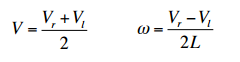
\includegraphics[width=1\hsize]{images/formula1.png}
\caption{Formula: Velocidade Linear (V), (W) Velocidade Rotacional ao longo do eixo}
\label{fig:fig1}
\end{figure}

Em que \(V_r\) é a velocidade da roda direita, \(V_l\) é a roda esquerda, \(D\) é a distância entre as rodas, \(V\) é a velocidade linear e \(\omega\) é a velocidade angular. 

\subsection{Pose}
A pose do robô é então calculada 

\begin{figure}[ht]
\centering
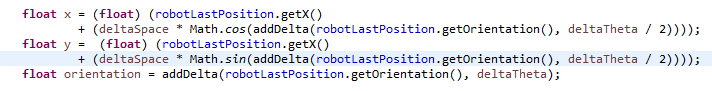
\includegraphics[width=1\hsize]{images/code-1.png}
\caption{Classe PositionLocator: odometry}
\label{fig:fig2}
\end{figure}


\subsection{Resultados dos testes}

Não foi possivel gerar o grafico de coordenadas das linhas de comparação, então determinei uma saída de console comparativa, somente para verificar a implementação e efetuar teste de que se havia erro acumulado.
A saida abaixo foi gerada ao usar o algoritmo para controle de Wall Follow, ap�s alguns algum tempo de execução:

\begin{figure}[ht]
\centering
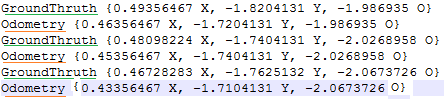
\includegraphics[width=1\hsize]{images/console-1.png}
\caption{Saida do console em vetor x,y, orientação, da PoseLocator}
\label{fig:fig3}
\end{figure}

Não consegui concluir com uma dimensão exata o acumulo erro cr�tico. Gostaria de gerar esses dados a partir de um grafico e conseguir tabelar o acumulo de erro. Para a pr�xima melhoria, irei implementar alguma alternativa para ter visualmente o caminho de cada posição percorrida e estimada do robô.
Logo se nota uma diferença após a execução por um minuto a minuto de execução, após a rotação do robô, o acumulo de diferença da odometria e do GroundThruth da posi��o real do robo. Para a implementação ser finalizada, necessita de uma correção de orientação usando-se algum outro enconder anexado ao robô Pioneer.


\section{Robot Fuzzy Control: Wall Follow - Seguir Parede}
A implementação da lógica fuzzy e do comportamento de seguir parede foi implementado na classe \textit{FuzzyWallFollower}. O controle tem por objetivo manter uma distância de 30cm da parede direita. A entrada do sistemas são apenas dois sensores do \textit{Pionner} modelados de acordo com a figura~\ref{fig:fig5}. A figura abaixo representa uma das modelagens usadas no sensor para o controle de wall following.
Pode-se ver todas as regras na classe (\textit{FuzzyWallFollower}). As figuras abaixo somente exemplificam a modelagem implementadas nas regras de entrada e sa�da e os exemplos de cada ativa��o.

\begin{figure}[ht]
\centering
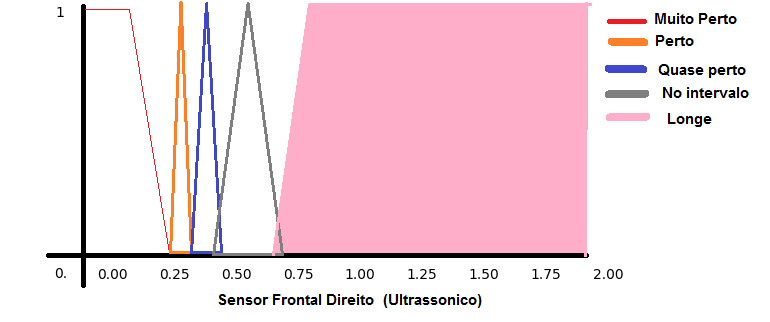
\includegraphics[width=1\hsize]{images/sensor-wall-follow-model.png}
\caption{Modelagem sensor frontal}
\label{fig:fig5}
\end{figure}

As saídas do sistema são a velocidade angular - figura~\ref{fig:fig6} - e a velocidade linear - figura~\ref{fig:fig7}. 

\begin{figure}[ht]
\centering
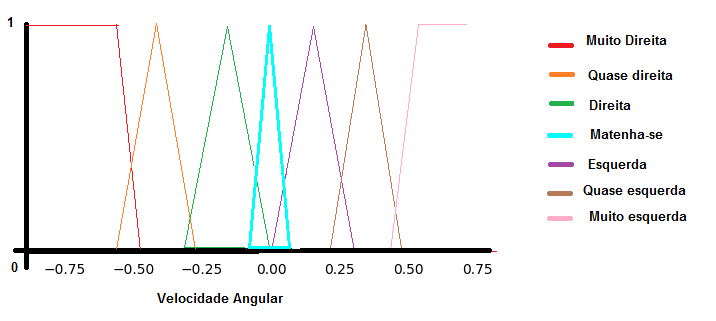
\includegraphics[width=1\hsize]{images/velocidade-angular-saida.png}
\caption{Modelagem Fuzzy da velocidade angular}
\label{fig:fig6}
\end{figure}

\begin{figure}[ht]
\centering
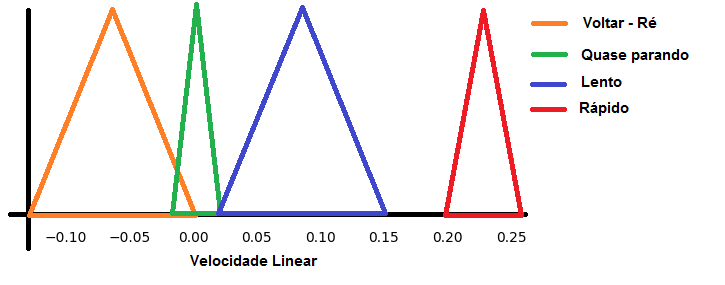
\includegraphics[width=1\hsize]{images/velocidade-linear-saida.png}
\caption{Modelagem velocidade linear}
\label{fig:fig7}
\end{figure}

\subsection{Resultados}

Os resultados se mostraram se promissores quando-se usado o fuzzy com uma modelagem correta, pode-se obter precisão nos comportamentos de execução dos algoritmos mencionados acima. Os resultados descritos nesse trabalho apenas foram exemplificações das implementações sugeridas ao decorrer do curso. Para cada implementação, obtive um teste básico para avaliar o aprendizado passado em sala de aula.
Porém ainda há alguns comportamentos a serem implementados e melhorados. O ajuste fino dessa modelagem necessita ser realizado caso queira que o comportamento do robô, se adapte-se ao ambiente sugerido para se completar tarefas com complexidade.
Não consegui evitar alguns problemas na simulação, como as passagens pelos obstaculos do cenário.
Porém creio que consegui o objetivo de entender a lógica de implementação dos algoritmos citados e consegui exemplifica-los na linguagem de programação Java.
Foram usados alguns artigos como leitura base de conhecimento das implementações realizadas ao longo da ultima década.Artigos \cite{Omrane:2016}, \cite{Beom:1995}.





%******************************************************************************
% Referências - Definidas no arquivo Relatorio.bib
 +-------------+

\bibliographystyle{IEEEtran}

\bibliography{Relatorio}


%******************************************************************************



\end{document}
